\documentclass[a4paper,12pt,titlepage,finall]{article}

\usepackage{amsmath}
\usepackage{amsfonts}
\usepackage{amssymb}\usepackage{amssymb}
\usepackage{csvsimple}
\usepackage{tikz}
\usepackage{pgfplots}
\usepackage{cmap}
\usepackage{color}
\usepackage[utf8x]{inputenc}
\usepackage[english,russian]{babel}
\usepackage[T2A]{fontenc}
\newcommand{\gt}{\textgreater} % знак больше
\newcommand{\lt}{\textless}       % знак меньше]
\usepackage[margin=2cm]{geometry}		 % для настройки размера полей
\usepackage{indentfirst}         % для отступа в первом абзаце секции
\usepackage{amsmath}
\usepackage{fancyvrb}
\usepackage{listings}
\usepackage{algorithm}
\usepackage{algpseudocode}
\usepackage{bm}
\usepackage{hyperref}

\usepackage{csvsimple}

\pgfplotsset{compat=1.11}
\usetikzlibrary{calc}
\lstset{
	inputencoding=utf8x,
	extendedchars=false,
	keepspaces = true,
	language=C++,
	basicstyle=\ttfamily,
	keywordstyle=\color[rgb]{0,0,1},
	stringstyle=\color[rgb]{0.627,0.126,0.941},
	numberstyle=\color[rgb]{0.205, 0.142, 0.73},
	frame=shadowbox,
	escapechar=`,
	numbers=left,
	breaklines=true,
	basicstyle=\ttfamily,
	literate={\ \ }{{\ }}1,
	tabsize=2,
	basicstyle=\footnotesize,
}
\lstset{language=C++,
	basicstyle=\ttfamily,
	keywordstyle=\color{blue}\ttfamily,
	stringstyle=\color{red}\ttfamily,
	%commentstyle=\color{green}\ttfamily,
	%morecomment=[l][\color{magenta}]{\#}
}
\DeclareMathOperator*{\EE}{\mathbb{E}}
\DeclareMathOperator*{\PP}{\mathbb{P}}
% выбираем размер листа А4, все поля ставим по 2см
\geometry{a4paper,left=20mm,top=20mm,bottom=20mm,right=20mm}

\setcounter{secnumdepth}{0}      % отключаем нумерацию секций

\begin{document}
	% Титульный лист
	\begin{titlepage}
		\begin{center}
			{\small \sc Московский государственный университет \\имени М.~В.~Ломоносова\\
				Факультет вычислительной математики и кибернетики\\}
			\vfill
			{\Large \sc Отчёт по заданию № 1}\\
		\end{center}
		\begin{flushright}
			\vfill {Выполнил:\\
				студент 317 группы\\
				Находнов~М.~С.\\
				~\\}
		\end{flushright}
		\begin{center}
			\vfill
			{\small Москва\\\the\year}
		\end{center}
	\end{titlepage}
		
% Автоматически генерируем оглавление на отдельной странице
\tableofcontents
\newpage
	
\begin{section}{Введение}
	В данном отчёте описаны  эксперименты, направленные на изучение качества и скорости работы алгоритма K-ближайших соседей (K-NN).\par
	Все эксперименты проведены на изображениях из датасета MNIST (60000 - размер обучающей выборки, 10000 - размер тестовой выборки).
\end{section}

\begin{section}{Эксперименты}
	
\begin{subsection}{Подбор параметра K}


\begin{table}[H]
	\begin{tabular}{c|c|c|c|c}
		N features & my\_own          & brute            & kd\_tree            & ball\_tree          \\
		\hline
		10         & $\bm{0.0}/48.65/48.65$ & $\bm{0.0}/15.83/15.83$  & $6.81/\bm{4.24}/\bm{11.05}$    & $6.53/5.74/12.27$    \\
		20         & $\bm{0.0}/70.78/70.78$ & $\bm{0.0}/16.58/16.59$  & $6.43/\bm{3.54}/\bm{9.97}$     & $6.18/14.36/20.54$   \\
		100        & $\bm{0.0}/73.03/73.03$ & $0.01/\bm{17.05}/\bm{17.06}$ & $6.72/177.03/183.75$ & $6.77/236.52/243.28$
	\end{tabular}
	\caption {Время работы различных алгоритмов в зависимости от размерности пространства признаков (fit time/predict time/fit + predict time). Измерения проводились усреднением по 3 независимым запускам}
	\label{tbl:1}
\end{table}
Из таблицы \ref{tbl:1} видно, что  при небольшой размерности пространства признаков kd\_tree и ball\_tree являются самыми быстрыми, однако, при увеличении размерности время работы алгоритмов, использующих деревья, значительно увеличивается и,  brute становится самым быстрым алгоритмом. В свою очередь, my\_own уступает brute в скорости работы. Это, вероятно, связано с тем, что brute использует реализацию K-NN из библиотеки sklearn, написанной на С, за счёт чего время исполнения программ, содержащих циклы значительно уменьшается.\par
Так как в дальнейшем тестирование будет происходить в пространстве признаков высокой размерности (728), то логично выбрать алгоритм brute, как самый быстрый и по времени обучения, и по времени поиска ближайших соседей.

\end{subsection}

\begin{subsection}{Подбор метрики и функции взвешивания}
	
\begin{figure}[H]
	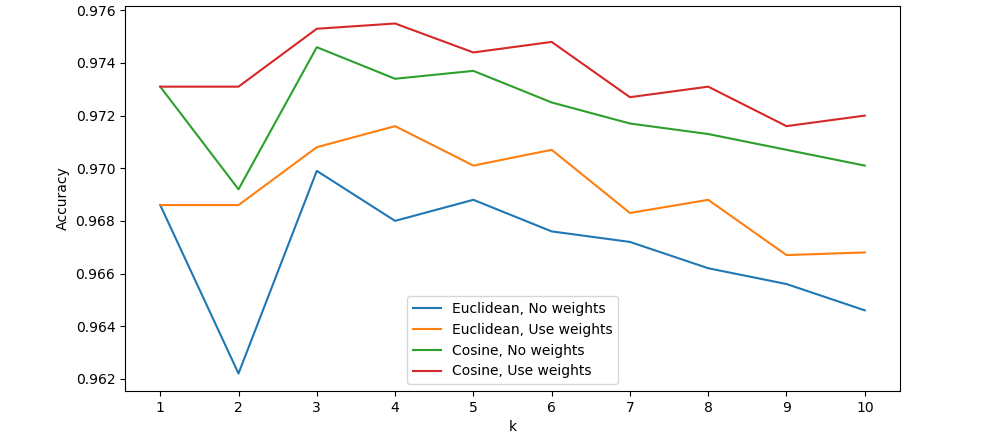
\includegraphics[scale=0.9]{\detokenize{./../experiment_2_3/scores_plot.png}}
	\centering
	\caption{Точность на тестовой выборке в зависимости от числа соседей, метрики и функции взвешивания}
	\label{pic:1}
\end{figure}

\begin{table}[H]
	\begin{tabular}{llll}
		Euclidean; No weights & Euclidean; Use weights & Cosine; No weights & Cosine; Use weights \\
		\hline
		$199.60$                & $193.57$                 & $413.96$             & $\bm{414.58}$             
	\end{tabular}
	\caption{Время работы алгоритмов в зависимости от используемой метрики и функции взвешивания. Замер производился на кросс валидации с 3 фолдами.}
	\label{tbl:2}
\end{table}
Алгоритм K-NN зависит от выбора метрики в пространстве признаков. Было рассмотрено две метрики --- евклидово расстояние и косинусное расстояние. Также, для вычисления предсказания алгоритм может использовать различные способы взвешивания ближайших соседей. Первый способ --- все соседи равнозначны и дают одинаковый вклад. Второй --- вес от соседа обратно пропорционален расстоянию между этим соседом и объектом тестовой выборки: $w_{i} = \frac{1}{||x - x_{i}|| + 10^{-5}}$.\par
Из рисунка \ref{pic:1} видно, что использование косинусного расстояния в качестве метрики значительно превосходит евклидову метрику вне зависимости от числа соседей. Добавление взвешивания с учётом расстояния между объектами тестовой и обучающей выборок позволяет улучшить точность как в случае евклидовой метрики, так и в случае косинусного расстояния. \par
Как следствие, для дальнейших экспериментов будет использоваться косинусная метрика, взвешивание объектов с четырьмя ближайшими соседями.\par
Однако, использование косинусной метрики замедляет время работы K-NN примерно в два раза \ref{tbl:2}. При этом взвешивание объектов с учётом расстояния не влияет на скорость работы.
\end{subsection}

\begin{subsection}{Анализ работы K-NN}

\begin{table}[H]
	\begin{tabular}{l|llllllllll}
		- & 0   & 1    & 2    & 3   & 4   & 5   & 6   & 7   & 8   & 9   \\
		\hline
		0 & 977 & 1    & 0    & 0   & 0   & 0   & 1   & 1   & 0   & 0   \\
		1 & 0   & 1129 & 3    & 1   & 0   & 0   & 2   & 0   & 0   & 0   \\
		2 & 8   & 0    & 1009 & 1   & 1   & 0   & 0   & 8   & 5   & 0   \\
		3 & 0   & 1    & 3    & 976 & 1   & $\bm{12}$  & 0   & 4   & $\bm{9}$   & 4   \\
		4 & 2   & 1    & 0    & 0   & 946 & 0   & 6   & 2   & 0   & $\bm{25}$  \\
		5 & 4   & 0    & 0    & $\bm{9}$   & 1   & 863 & 7   & 1   & 4   & 3   \\
		6 & 3   & 3    & 0    & 0   & 1   & 3   & 948 & 0   & 0   & 0   \\
		7 & 2   & $\bm{10}$   & 4    & 0   & 1   & 0   & 0   & 998 & 0   & $\bm{13}$  \\
		8 & 7   & 1    & 2    & $\bm{9}$   & 3   & 3   & 5   & 4   & 936 & 4   \\
		9 & 7   & 7    & 2    & 5   & 7   & 3   & 1   & 4   & 3   & 970
	\end{tabular}
	\centering
	\caption{Confution matrix, 4-NN, Cosine with weights}
	\label{tbl:3}
\end{table}
	
\begin{table}[H]
	\begin{tabular}{ccc}
		Test   & SOTA   & Cross validation \\
		\hline
		0.9752 & 0.9979 & 0.9755          
	\end{tabular}
	\centering
	\caption{Точность на тестовой выборке с помощью 4-NN; лучший достигнутый результат \cite{MNISTSOTA}; точность на кроссвалидации с помощью 4-NN}
	\label{tbl:4}
\end{table}

Таблица \ref{tbl:4}, показывает, что оценка полученная на кросс валидации близка к оценке на тестовой выборке. Это говорит о том, что подбор параметров с помощью обучающей выборки на кросс валидации не приводит к переобучению. При этом лучший результат, полученный с помощью K-NN, значительно (на $4.5\%$) уступает state-of-the-art результатам. \par
Из confution matrix \ref{tbl:3} видно, что наибольшее число ошибок допускается на визуально похожих объектах, например, 4 и 9, 3 и 8, 7 и 1. Рисунок \ref{pic:1} показывает, что ошибки классификации  происходят на тех объектах, где цифра изображена, или неразборчиво, или похожей по начертанию на другую цифру.

\begin{figure}[H]
	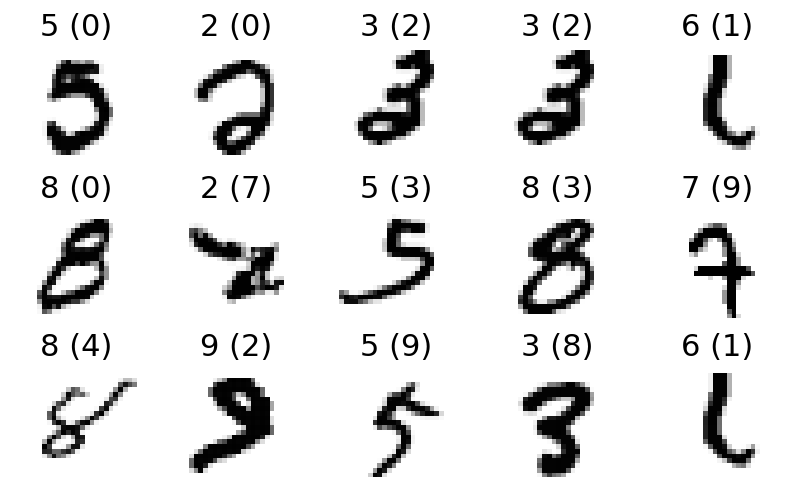
\includegraphics[scale=0.75]{\detokenize{./../experiment_4/wrong_classifies.png}}
	\centering
	\caption{Неверно классифицированные объекты. Корректная метка (Предсказанная метка)}
	\label{pic:1}
\end{figure}


\end{subsection}
	
\begin{subsection}{Аугментация}
	
\begin{table}[H]
	\begin{tabular}{c||c|c}
		- & Train transformation & Test tranformation \\
		\hline
		Rotation, $angle=5$          & $0.9765$               & $0.9764$             \\
		Rotation, $angle=10$         & $0.9802$               & $\bm{0.9796}$             \\
		Rotation, $angle=15$         & $0.9785$               & $0.9781$             \\
		Shift, $x\_shift=y\_shift = 1$ & $0.9760$               & $0.9760$             \\
		Shift, $x\_shift=y\_shift = 2$ & $0.9756$               & $0.9756$             \\
		Shift, $x\_shift=y\_shift = 3$ & $0.9752$               & $0.9752$             \\
		Blur, $sigma=0.5$          & $0.9758$               & $0.9729$             \\
		Blur, $sigma=1.0$          & $\bm{0.9814}$               & $0.9632$             \\
		Blur, $sigma=1.5$          & $0.9782$               & $0.9278$            
	\end{tabular}
	\centering
	\label{tbl:5}
	\caption{Точность в результате трансформации обучающей или тестовой выборки}
\end{table}

<<Размножение>> выборки, как обучающей, так тестовой (за исключением размытия) или улучшает качество (повороты), или оставляет его без изменения (сдвиги). \par
Ожидаемо, что линейные трансформации дают одинаковый эффект, что при применении к обучающей, что при применении к тестовой выборке. Это связано с тем, что, например, для поворотов в выборку добавляются как повороты на лево, так и направо с одним и тем же углом поворота. Небольшое отличие в точности, связано с тем, что при поиске k ближайших соседей для аугментированной тестовой выборки, находился список из k соседей для каждого варианта изменения тестового объекта. Затем эти списки объединялись и выбирались k ближайших объектов. Такой подход допускал повторения соседей в итоговом списке k ближайших соседей.\par
	
Рассмотрим те классы для которых K-NN стал давать больше правильных ответов. Для этого рассмотрим лучшее из всех преобразований (blur, $sigma=1.0$, train transformation) и построим разность исходной confution matrix и матрицы после применения аугментации
\begin{table}[H]
	\begin{tabular}{c|cccccccccc}
		- & 0  & 1  & 2  & 3  & 4  & 5  & 6  & 7 & 8  & 9   \\
		\hline
		0 & 0  & 0  & 0  & 0  & 0  & 0  & -1 & 1 & 0  & 0   \\
		1 & 0  & 1  & 0  & -1 & 0  & 0  & 0  & 0 & 0  & 0   \\
		2 & -1 & 1  & -3 & 1  & 0  & 0  & 1  & 4 & -3 & 0   \\
		3 & 0  & -1 & -2 & $10^*$ & 0  & -3 & 0  & 0 & -4 & 0   \\
		4 & -2 & -1 & 0  & 0  & $14^*$ & 0  & -2 & 1 & 0  & $\bm{-10}$ \\
		5 & -2 & 1  & 0  & -3 & 0  & 9  & -3 & 0 & -2 & 0   \\
		6 & 0  & 0  & 0  & 0  & 0  & 0  & 0  & 0 & 0  & 0   \\
		7 & -2 & -3 & 2  & 0  & 2  & 1  & 0  & 5 & 0  & -5  \\
		8 & -4 & -1 & -1 & $\bm{-6}$ & 0  & 0  & -2 & 0 & $15^{*}$ & -1  \\
		9 & $\bm{-5}$ & -3 & -2 & -3 & 1  & 0  & 0  & 2 & -1 & $11^*$ 
	\end{tabular}
	\centering
	\caption{Разность confution matrix до и после аугментации.}
	\label{tbl:6}
\end{table}

Как видно из таблицы \ref{tbl:6} наибольшие улучшения произошли для классов 4 и 9, 3 и 8, 0 и 9 --- классы, которые могут быть сложно отличимы друг от друга даже визуально. При этом, применение размытия больше всего повлияло на классы, в которых цифры имеют <<округлые>>, выпуклые части (3, 8, 9).
\begin{figure}[H]
	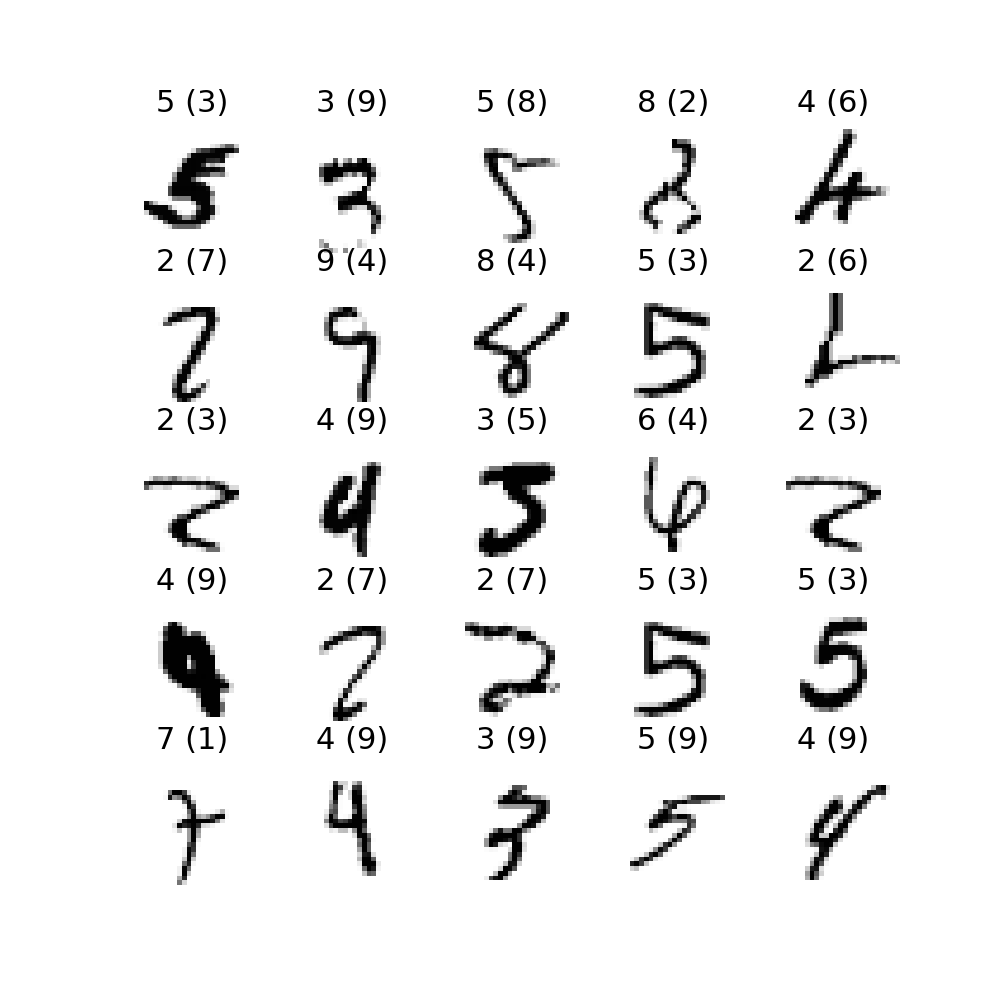
\includegraphics[scale=0.75]{\detokenize{./../experiment_5/wrong_classifies_blur.png}}
	\centering
	\caption{Неверно классифицированные объекты. Корректная метка (Предсказанная метка)}
	\label{pic:2}
\end{figure}

Изучение неверно классифицированных объектов (рис. \ref{pic:2}) показывает, что наиболее часто ошибки происходят на цифрах, где нечёткое написание петелек или стиль написания цифры (например 1 и 7) делает затруднительным определение правильного класса даже человеку. \par

Несмотря на то, что применение размытия к обучающей выборке приводит к наибольшему увеличению точности классификации, однако, применение аналогичного преобразования к тестовой выборке напротив значительно ухудшает качество работы.\par

При этом, как было сказано ранее, при применении линейных трансформаций разницы между аугментацией тестовой выборки и аугментации обучающей выборки нет, но при этом, аугментация тестовой выборки работает значительно быстрее, чем аугментация обучающей выборки.\par

Итого, можно сказать, что аугментация данных может как улучшать качество, так и ухудшать качество и, как следствие, на практике правильный метод изменения данных следует подбирать как гиперпараметр, оценивая качество, например, по кросс валидации.

\end{subsection}
	
\end{section}

\begin{section}{Выводы}
	Алгоритм K-NN показал, что он может применяться для задачи классификации изображений и достигать приемлемой точности. Однако, от правильного выбора гиперпараметров (алгоритма поиска ближайших соседей, числа ближайших соседей, метрики, функции взвешивания, вида аугментации) существенно зависит как скорость работы алгоритма, так качество классификации тестовой выборки.
\end{section}

\newpage

\begin{thebibliography}{9}
	\bibitem{MNISTSOTA} \detokenize{http://rodrigob.github.io/are_we_there_yet/build/classification_datasets_results.html}
\end{thebibliography}


\end{document}